\chapter{Methodology}
We are planning to implement our project in three phases.In the initial phase we analyse the requirements needed for this by reading many papers related to this topic.From the papers we read we get knowledge about many things.We design a system from the knowledge we acquired.In the second phase we design a interface for chatting which is very useful for users of the website with another user.we also design a interface for rate and review to review the website.Then we collect data and prepare the data by identifying incomplete,incorrect,inaccurate and deleting corrupt data.By machine learning we train the data to train an algorithm to predict the outcome of the design.Then we test the data to evaluate the performance and improve the results.To evaluate the performance we also learn and validate the data.We decided to do this by dividing our group into two.One group design interface for chat,rate and other group prepare the data.In the final phase we combine all these modules and deploy it.
\pagebreak


\begin{figure}
    \centering
    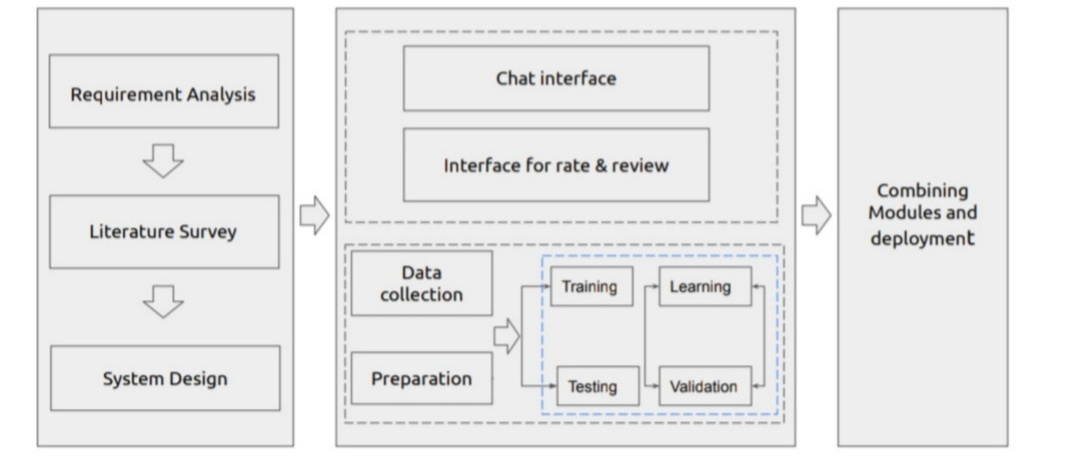
\includegraphics[scale=0.5]{images/project_phases.jpeg}
    \caption{Project phases}
    \label{fig:Methodology}
\end{figure}


